\documentclass{beamer}
\usepackage{graphicx}
\usepackage{xcolor}
\usepackage{tikz}
\usepackage{amsmath}

\definecolor{purpleblue}{RGB}{80, 80, 180}
\definecolor{novelPurple}{RGB}{98, 54, 255}
\definecolor{softPurple}{RGB}{180, 170, 255}
\definecolor{softGray}{RGB}{235, 235, 245}
\definecolor{lightText}{RGB}{90, 90, 110}

\usetheme{Madrid}
\usecolortheme{dolphin}
\graphicspath{{static/course_materials/}{static/hard/}{./}}

\setbeamerfont{title}{size=\Large,series=\bfseries}
\setbeamerfont{frametitle}{size=\LARGE,series=\bfseries}
\setbeamercolor{frametitle}{fg=white, bg=novelPurple}
\setbeamercolor{title}{fg=white, bg=purpleblue}

\title[SAT Hard Question 7]{\textbf{SAT Hard Question\\ Set 7}}
\author{\textbf{Jack Zeng}}
\institute{\textcolor{white}{\textbf{Novel Prep}}}
\date{\today}

\begin{document}

\begin{frame}
    \titlepage
    \vfill
    \begin{flushright}
        \textcolor{purpleblue}{\Huge \textbf{Novel Prep}}
    \end{flushright}
\end{frame}

\begin{frame}
    \begin{tikzpicture}[remember picture, overlay]
        \shade[top color=softPurple, bottom color=softGray]
            (current page.north west) rectangle (current page.south east);
        \node[align=center] at (current page.center) {
            {\Huge\bfseries\textcolor{purpleblue}{Novel Prep}} \\[0.5cm]
            {\Large\itshape\textcolor{lightText}{Phase 2 · Hard Question Practice}}
        };
    \end{tikzpicture}
\end{frame}

\begin{frame}{Overview}
    \tableofcontents
\end{frame}

\begin{frame}
\section{Hard Question Set 7}
    \begin{tikzpicture}[remember picture, overlay]
        \shade[top color=softPurple, bottom color=softGray]
            (current page.north west) rectangle (current page.south east);
        \node[align=center] at (current page.center) {
            {\LARGE\bfseries\textcolor{purpleblue}{Hard Question Set 7}} \\[0.5cm]
            {\Large\itshape\textcolor{lightText}{12 SAT-style challenge problems}}
        };
    \end{tikzpicture}
\end{frame}

% --- Question 1 ---
\begin{frame}{Question 1}
\small
A rectangular region of land is divided into 54 square lots of equal area \(S\) in square units. The length of the region is 1.5 times the width of the region. If the width of the region is \(a\sqrt{S}\) units, what is the value of \(a\)?
\vspace{0.35cm}
\begin{enumerate}
    \item[A.] 5
    \item[B.] 6
    \item[C.] 7
    \item[D.] 8
\end{enumerate}
\end{frame}
\begin{frame}{Answer 1}
\small
\textbf{Correct Answer:} B
\end{frame}

% --- Question 2 ---
\begin{frame}{Question 2}
\small
In the given pair of equations, \(a\) and \(b\) are constants. The graph of this pair of equations in the \(xy\)-plane is a pair of perpendicular lines.

Which of the following pairs of equations also represents a pair of perpendicular lines?
\[
\begin{aligned}
5x + 7y &= 1 \\
ax + by &= 1
\end{aligned}
\]
\vspace{0.35cm}
\begin{enumerate}
    \item[A.] \(10x + 7y = 1\), \(ax - 2by = 1\)
    \item[B.] \(10x + 7y = 1\), \(ax + 2by = 1\)
    \item[C.] \(10x + 7y = 1\), \(2ax + by = 1\)
    \item[D.] \(5x - 7y = 1\), \(ax + by = 1\)
\end{enumerate}
\end{frame}
\begin{frame}{Answer 2}
\small
\textbf{Correct Answer:} B
\end{frame}

% --- Question 3 ---
\begin{frame}{Question 3}
\small
A real estate company offers a series of three webinars. 2,000 people attended the first webinar. 65\% of the people who attended the first webinar attended the second webinar, and 44\% of the people who attended both the first and second webinars attended the third webinar.

If those who attended the first but did not attend the second webinar, 31\% attended the third webinar.

How many people attended both the first and third webinars but did not attend the second webinar?
\vspace{0.35cm}
\begin{enumerate}
    \item[A.] 215
    \item[B.] 217
    \item[C.] 219
    \item[D.] 220
\end{enumerate}
\end{frame}
\begin{frame}{Answer 3}
\small
\textbf{Correct Answer:} B
\end{frame}

% --- Question 4 ---
\begin{frame}{Question 4}
\small
The functions \(f\) and \(g\) are defined by the given equations, where \(x \geq 0\):

\begin{itemize}
\item[I] \(f(x) = 19(1.27)^x + 43\)
\item[II] \(g(x) = 8(0.77)^x\)
\end{itemize}

Which of the following equations displays, as a constant or coefficient, the maximum value of the function it defines, where \(x \geq 0\)?
\vspace{0.35cm}
\begin{enumerate}
    \item[A.] I only
    \item[B.] II only
    \item[C.] I and II
    \item[D.] Neither I nor II
\end{enumerate}
\end{frame}
\begin{frame}{Answer 4}
\small
\textbf{Correct Answer:} B
\end{frame}

% --- Question 5 ---
\begin{frame}{Question 5}
\small
Circle \(F\) in the \(xy\)-plane is represented by the equation:
\[
(x - 13)^2 + (y - 9)^2 = 196
\]
Circle \(G\) is obtained by shifting circle \(F\) 5 units to the left and 11 units up. An equation representing circle \(G\) is:
\[
(x + h)^2 + (y + k)^2 = 196
\]
where \(h\) and \(k\) are constants.

What is the value of \(h + k\)?
\end{frame}
\begin{frame}{Answer 5}
\small
\textbf{Final Answer:} $\boxed{-28}$
\end{frame}

% --- Question 6 ---
\begin{frame}{Question 6}
\small
The function \(q\) is defined by:
\[
q(x) = a|x - 9|^2 - 87|x - 9| + b
\]
where \(a\) and \(b\) are constants, and \(a > b > 87\).

If \(q(639) = h\) and \(q(-621) = k\), where \(h\) and \(k\) are constants, what is the value of:
\[
9(-639)^{h-k} + 621(9)^{k-h}?
\]
\end{frame}
\begin{frame}{Answer 6}
\small
\textbf{Final Answer:} $\boxed{630}$
\end{frame}

% --- Question 7 ---
\begin{frame}{Question 7}
\small
In the given equation, \(a\) and \(b\) are positive constants. A solution to the equation is \(x = 42\).
\[
x(9x - 2a) + b(9x - 2a) - (x + b) = 0
\]
What is the value of \(a\)?
\end{frame}
\begin{frame}{Answer 7}
\small
\textbf{Final Answer:} $\boxed{188.5}$
\end{frame}

% --- Question 8 ---
\begin{frame}{Question 8}
\small
A right rectangular prism has a base area of \(28p\) square centimeters (\(\text{cm}^2\)). The length of the base of the rectangular prism is 12 cm, and the height of the rectangular prism is 4 cm.

Which expression represents the surface area, in \(\text{cm}^2\), of the right rectangular prism?
\vspace{0.35cm}
\begin{enumerate}
    \item[A.] \(\dfrac{512p}{3}\)
    \item[B.] \(\dfrac{224p}{3} + 96\)
    \item[C.] \(56p + 192\)
    \item[D.] \(560p + 96\)
\end{enumerate}
\end{frame}
\begin{frame}{Answer 8}
\small
\textbf{Correct Answer:} B
\end{frame}

% --- Question 9 ---
\begin{frame}{Question 9}
\small
The expression
\[
\frac{x^{-2}y^{\frac{1}{2}}}{x^{\frac{1}{3}} y^{-1}}
\]
where \(x > 1\) and \(y > 1\), is equivalent to which of the following?
\vspace{0.35cm}
\begin{enumerate}
    \item[A.] \(\dfrac{\sqrt{y}}{\sqrt[3]{x}}\)
    \item[B.] \(\dfrac{y\sqrt{y}}{\sqrt[3]{x}}\)
    \item[C.] \(\dfrac{y\sqrt{y}}{x\sqrt[3]{x}}\)
    \item[D.] \(\dfrac{y\sqrt{y}}{x^2\sqrt[3]{x}}\)
\end{enumerate}
\end{frame}
\begin{frame}{Answer 9}
\small
\textbf{Correct Answer:} D
\end{frame}

% --- Question 10 ---
\begin{frame}{Question 10}
\small
The function \(z\) is defined by the equation:
\[
z(w) = (0.829)^{2w}
\]
The value of \(z(w)\) decreases by \(p\%\) for each increase by 1 in the value of \(w\). Which of the following is closest to the value of \(p\)?
\vspace{0.35cm}
\begin{enumerate}
    \item[A.] 0.171
    \item[B.] 0.829
    \item[C.] 17.1
    \item[D.] 31.3
\end{enumerate}
\end{frame}
\begin{frame}{Answer 10}
\small
\textbf{Correct Answer:} D
\end{frame}

% --- Question 11 ---
\begin{frame}{Question 11}
\small
\[
-16(5x - 3)^2 + 4(5x - 2)^2
\]
The given expression can be rewritten as:
\[
\frac{a}{4}x^2 + \frac{b}{4}x + \frac{c}{4}
\]
where \(a, b,\) and \(c\) are constants. What is the value of \(a + b + c\)?
\vspace{0.35cm}
\begin{enumerate}
    \item[A.] -112
    \item[B.] -56
    \item[C.] -28
    \item[D.] -7
\end{enumerate}
\end{frame}
\begin{frame}{Answer 11}
\small
\textbf{Correct Answer:} A
\end{frame}

% --- Question 12 ---
\begin{frame}{Question 12}
\small
\begin{center}
    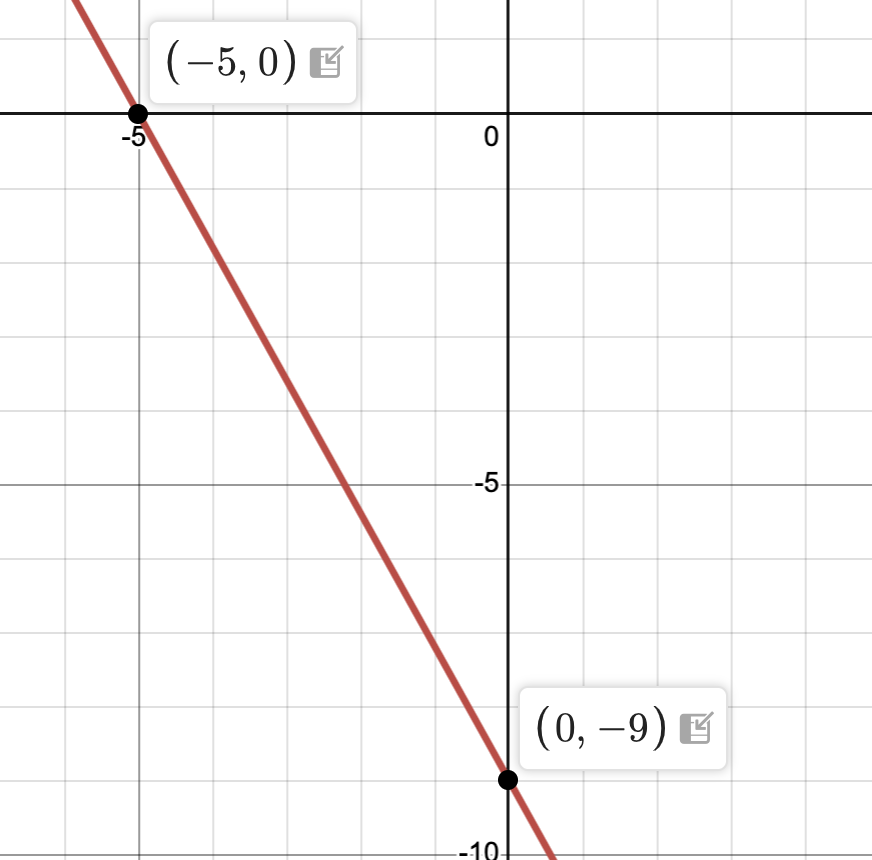
\includegraphics[width=0.42\linewidth]{hard_7_f4.png}
\end{center}

The graph of line \(h\) is shown in the \(xy\)-plane. Line \(k\) (not shown) is defined by the equation:
\[
sx + 40y = t
\]
where \(s\) and \(t\) are constants. If line \(k\) is graphed in this \(xy\)-plane, the result is a graph of two linear equations. This system of two linear equations has no solution.

Which of the following is \textbf{NOT} a possible value of \(t\)?
\vspace{0.35cm}
\begin{enumerate}
    \item[A.] -360
    \item[B.] -9
    \item[C.] 72
    \item[D.] 200
\end{enumerate}
\end{frame}
\begin{frame}{Answer 12}
\small
\textbf{Correct Answer:} A
\end{frame}

\begin{frame}{}
    \begin{tikzpicture}[remember picture, overlay]
        \shade[top color=novelPurple!40, bottom color=white]
            (current page.north west) rectangle (current page.south east);
        \fill[white, opacity=0.15] (current page.center) circle (5cm);
        \foreach \x in {1,2,3,4,5} {
            \fill[novelPurple, opacity=0.12] (rand*10-5, rand*7-3.5) circle (0.1+\x*0.05);
        }
    \end{tikzpicture}
    \centering
    \vspace{5em}
    {\Huge \textbf{\textcolor{novelPurple}{Thank You!}}} \\[1em]
    {\large \textcolor{gray}{We appreciate your time and focus.}} \\[3em]
    {\LARGE \textbf{\textcolor{novelPurple}{\textsf{Novel Prep}}}}
    \vfill
\end{frame}

\end{document}
